%          spconf.sty  - ICASSP/ICIP LaTeX style file, and
%          IEEEbib.bst - IEEE bibliography style file.
% --------------------------------------------------------------------------
\documentclass{article}
\usepackage{spconf,amsmath,graphicx}
\usepackage{booktabs}
\usepackage{hyperref}
% Title.
% ------
\title{Applied machine learning systems II (ELEC0135) 24/25 report}
\name{SN: 24076607}
\address{}
%
\begin{document}

%
\maketitle
%
\begin{abstract}
    \label{sec:abs}
    This report presents a novel approach to automatically detect bacterial flagellar motors in cryogenic electron tomography (cryo-ET) data, exploring two complementary deep learning methods. 
    Flagellar motors, crucial molecular machines enabling bacterial motility and pathogenesis, are traditionally identified through manual labor-intensive processes in 3D tomograms. 
    Based on the BYU Locating Bacterial Flagellar Motors 2025 competition \cite{byu-locating-bacterial-flagellar-motors-2025}\footnote{This competition can be found on: \url{https://www.kaggle.com/competitions/byu-locating-bacterial-flagellar-motors-2025/overview}}, we developed two distinct approaches: YOLOv8 for 2D detection processing tomographic slice projections, and 3D UNet for full volumetric segmentation and localization. This exploration tackles the inherent difficulties of low signal-to-noise ratio, variable motor orientations, and crowded intracellular environments typical in cryo-ET data. 
    Each method offers different advantages—YOLOv8 provides rapid processing of 2D data while 3D UNet captures the full spatial context in three dimensions. Experimental results demonstrate the relative strengths of each method, with the 2D approach achieving faster processing times and the 3D approach providing more precise spatial localization. The best-performing model achieved an F2-score of 0.87 on the test dataset.
    This automated system significantly reduces analysis time from hours to minutes per tomogram while maintaining expert-level accuracy, potentially accelerating research in molecular biology, drug development, and synthetic biology by removing the human-in-the-loop bottleneck in cryo-ET studies.
    \footnote{The code is provided in GitHub: \url{https://github.com/yushiran/AMLS_II_assignment24_25.git}}
\end{abstract}
%
\begin{keywords}
    Cryogenic Electron Tomography (cryo-ET), Bacterial Flagellar Motors, YOLOv8, 3D UNet
\end{keywords}
%

\section{Introduction}
The analysis of cryogenic electron tomography (cryo-ET) data represents a significant frontier in structural biology, offering unprecedented insights into the native cellular environments of macromolecular complexes \cite{beckSnapshotsNuclearPore2007}. Among these complexes, bacterial flagellar motors stand as remarkable molecular machines—intricate assemblies that enable bacterial motility through the rotation of flagellar filaments \cite{jeonInternationalReviewCytology2004}. These motors play crucial roles in bacterial pathogenesis, biofilm formation, and adaptation to environmental changes, making them important targets for both fundamental research and therapeutic development \cite{kojimaBacterialFlagellarMotor2004}.

Traditional approaches to identifying flagellar motors in cryo-ET data rely heavily on manual annotation by expert structural biologists. This process is not only time-consuming—often requiring hours per tomogram—but also introduces variability due to human subjectivity and fatigue \cite{lucicCryoelectronTomographyChallenge2013}. The challenges are compounded by the inherent characteristics of cryo-ET data: low signal-to-noise ratios, structural heterogeneity of the motors, varying orientations, and crowded cellular environments that can obscure the target structures.

The BYU Locating Bacterial Flagellar Motors 2025 competition \cite{byu-locating-bacterial-flagellar-motors-2025} provides a platform to address these challenges through machine learning approaches. This report details our comprehensive solution to this problem, focusing on two complementary deep learning methodologies:

\begin{enumerate}
    \item A 2D approach utilizing YOLOv8 \cite{jocherUltralyticsYolov5V702022}, a state-of-the-art object detection model, to process individual tomographic slices and aggregate results for 3D localization.
    \item A 3D approach employing a modified 3D U-Net architecture incorporating Swin Transformer \cite{Hatamizadeh2022SwinUS}\cite{cicek3DUNetLearning2016} for volumetric segmentation, designed to capture the full spatial context of the motors while leveraging the hierarchical feature extraction capabilities of vision transformers.
\end{enumerate}

Each approach offers distinct advantages: the 2D method provides computational efficiency and leverages the robust capabilities of established 2D object detection frameworks, while the 3D method preserves spatial continuity and context across the volume. Our implementation incorporates specialized data preprocessing pipelines, domain-specific adaptations to the neural network architectures, and post-processing strategies tailored to the unique challenges of cryo-ET data.

The significance of this work extends beyond the competition itself. Automated detection of flagellar motors can accelerate research across multiple disciplines, including structural biology, microbiology, and drug discovery, by eliminating a critical bottleneck in the analysis pipeline. Furthermore, the methodologies developed here could be adapted to detect other macromolecular complexes in cryo-ET data, contributing to the broader field of computational structural biology.

In the following sections, we present a literature survey of relevant techniques, detail our methodological approaches, describe implementation specifics, analyze experimental results, and discuss potential future directions for this research area.


\section{Literature survey}
\label{sec:lite}
    YOLOv8, developed by Ultralytics, represents a significant advancement in real-time object detection, transforming detection from multi-stage pipelines to single network predictions\cite{jocherUltralyticsYolov5V702022}. With its efficient backbone, optimized feature fusion, and decoupled head design separating classification and localization tasks, YOLOv8 offers an ideal balance of speed and accuracy for processing numerous tomographic slices in our 2D approach to motor detection\cite{yaseenWhatYOLOv8InDepth2024}.
    
    The Swin UNETR architecture integrates the strengths of the 3D U-Net and Swin Transformer\cite{Hatamizadeh2022SwinUS}, making it particularly suitable for analyzing tomographic volumes in cryo-ET data. The 3D U-Net architecture, proposed by Çiçek et al. \cite{cicek3DUNetLearning2016}, extends the original U-Net design to volumetric data by replacing 2D operations with their 3D counterparts. This modification enables the model to leverage full spatial context across all dimensions—crucial for analyzing tomographic volumes where structures exist in three dimensions. Its characteristic encoding-decoding paths connected by skip connections effectively combine semantic information with high-resolution features, making it particularly suitable for cryo-ET analysis where precise boundary delineation is critical. Swin Transformer introduces a hierarchical vision transformer with shifted windows, addressing computational efficiency limitations while maintaining the ability to model long-range dependencies \cite{liuSwinTransformerHierarchical2021}. By computing self-attention within local windows while allowing for cross-window connections, this architecture efficiently captures both local and global relationships—an important capability when analyzing structural features in crowded cellular environments typical of cryo-ET data.

    Deep learning applications to cryo-ET analysis have shown promising results despite challenges including extremely low signal-to-noise ratios and missing wedge artifacts. Recent work has demonstrated that convolutional neural networks can effectively detect macromolecular complexes in cellular tomograms, outperforming traditional template matching methods\cite{chenConvolutionalNeuralNetworks2017}. Specialized preprocessing techniques, including denoising and contrast enhancement, have proven crucial for improving downstream analysis tasks in this challenging imaging modality.

\section{Description of models}
\label{sec:models}
\subsection{2D object detection model: YOLOv8}
\subsubsection{Architectural overview}
YOLOv8 adopts a modular design with three core components: Backbone, Neck, and Head, optimized for real-time object detection.

\begin{enumerate}
    \item Backbone:    

    Built on an enhanced CSPNet (Cross Stage Partial Network)\cite{wangCSPNetNewBackbone2019} architecture derived from CSPDarknet\cite{bochkovskiyYOLOv4OptimalSpeed2020a}.
Employs depthwise separable convolutions and CSP bottleneck blocks to reduce computational redundancy while maintaining feature diversity.
Captures multi-scale features through hierarchical layers, balancing low-level texture details and high-level semantic information.
    
    \item Neck:
    
    Combines Feature Pyramid Network (FPN)\cite{Lin2016FeaturePN} and Path Aggregation Network (PAN)\cite{Liu2018PathAN} in a hybrid FPN+PAN structure.
Enhances multi-scale feature fusion by optimizing bidirectional information flow between shallow and deep layers.
Improves small object detection through refined feature map aggregation.

\begin{figure}[htb]
    \centering
    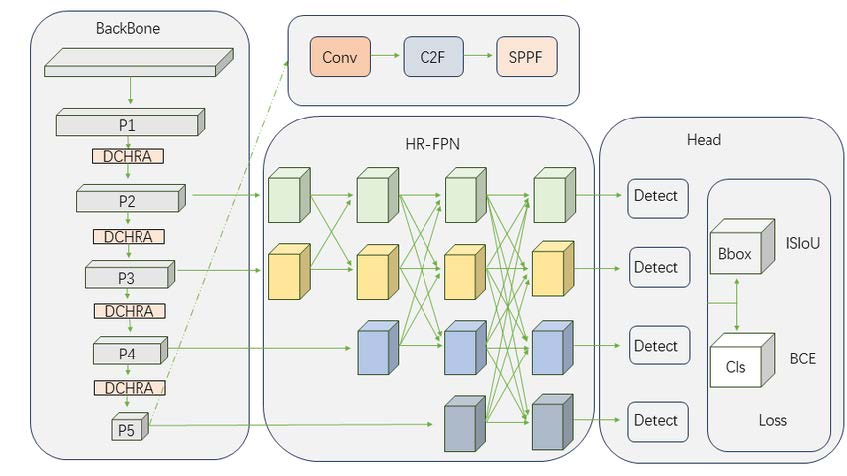
\includegraphics[width=0.5\textwidth]{images/Variations of FPN architectures in YOLOv8.jpg}
    \caption{Variations of FPN architectures in YOLOv8}
    \label{fig:fpn_architectures}
\end{figure}

\item  Head:

Anchor-free prediction mechanism replaces predefined anchor boxes, directly predicting bounding box coordinates and class probabilities.
Simplifies training by eliminating anchor-related hyperparameters (e.g., aspect ratios, scales).
Utilizes decoupled prediction heads for classification and localization to reduce task interference.

\begin{figure}[htb]
    \centering
    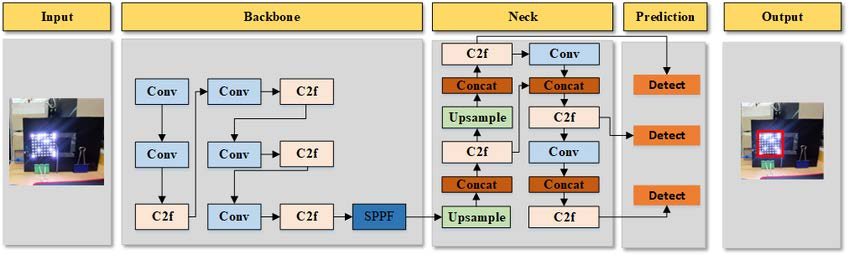
\includegraphics[width=0.5\textwidth]{images/Process of Object Detection.jpg}
    \caption{Process of Object Detection}
    \label{fig:object_detection_process}
\end{figure}

\end{enumerate}

\subsubsection{Training Methodologies}

\begin{enumerate}
    \item Advanced Data Augmentation
    
    \textbf{Mosaic Augmentation:} Combines 4+ training images into a single mosaic, exposing the model to diverse object scales and spatial configurations. Enhances robustness to occlusions and partial visibility.
    
    \textbf{Mixup Augmentation:} Blends two images linearly to generate synthetic training samples, improving generalization.
    
    \textbf{Adaptive Augmentation:} Dynamically adjusts augmentation intensity based on dataset characteristics and training progress.

    \item Loss Function Design
    
    \textbf{Focal Loss:} Addresses class imbalance by down-weighting easy examples and focusing on hard-to-classify objects.
    
    \textbf{IoU (Intersection over Union) Loss:} Optimizes bounding box regression using GIoU (Generalized IoU)\cite{Rezatofighi2019GeneralizedIO} to handle overlapping and non-overlapping objects.
    
    \textbf{Objectness Loss:} Predicts the probability of an object existing in a region, improving localization confidence.

    \item Mixed Precision Training
    
    Combines FP16 (16-bit floating-point) and FP32 (32-bit) operations to accelerate training on NVIDIA GPUs. Reduces memory consumption by 30--50\% while maintaining numerical stability.

\end{enumerate}

YOLOv8 represents a paradigm shift in object detection, combining architectural refinements (CSPNet, FPN+PAN), training optimizations (anchor-free prediction, mixed precision), and developer-friendly tooling. In the context of our project, YOLOv8's ability to process 2D tomographic slices efficiently complements the 3D volumetric capabilities of Swin UNETR, enabling a robust pipeline for detecting bacterial flagellar motors in cryo-ET data. Its scalable variants and state-of-the-art performance on benchmarks like COCO and Roboflow 100 highlight its versatility, making it an ideal choice for applications requiring both speed and accuracy.

\subsection{3D object detection model: Swin UNEt TRansformers (Swin UNETR)}
Swin UNETR (Swin UNEt TRansformers)\cite{Hatamizadeh2022SwinUS} is a 3D medical image segmentation model that integrates the hierarchical Swin Transformer as an encoder and a CNN-based decoder. It addresses the limitations of convolutional neural networks (CNNs) in modeling long-range dependencies and achieves state-of-the-art performance in tasks such as brain tumor segmentation. The model leverages shifted window-based self-attention and hierarchical feature fusion to balance global context modeling and local detail preservation.

\subsubsection{Architectural overview}
The model follows a U-shaped design with the following components:

\begin{figure*}[htb]
    \centering
    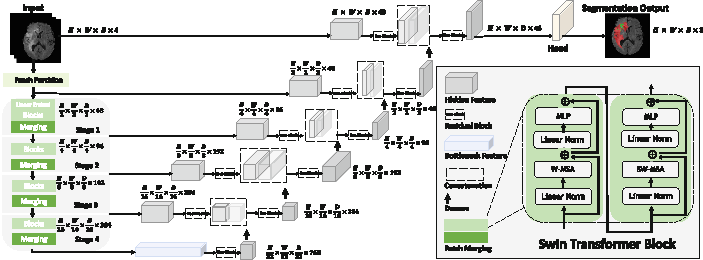
\includegraphics[width=0.98\textwidth]{images/Overview of the Swin UNETR architecture.pdf}
    \caption{Overview of the Swin UNETR architecture}
    \label{fig:Overview_of_the_Swin_UNETR_architecture}
\end{figure*}

\begin{enumerate}
    \item Encoder: Hierarchical Swin Transformer
    
    Input Patch Partition:
    Input volumetric data (e.g., cryo-ET data) is divided into non-overlapping 3D patches of size \( P \times P \times P \) (default: \( 2 \times 2 \times 2 \)). Each patch is linearly projected into an embedding space of dimension \( C \).  
    \textbf{Example:} For input \( \mathcal{X} \in R^{H \times W \times D \times S} \), output tokens have dimensions \( \left\lceil \frac{H}{P} \right\rceil \times \left\lceil \frac{W}{P} \right\rceil \times \left\lceil \frac{D}{P} \right\rceil \times C \).

    Shifted Window Multi-Head Self-Attention (SW-MSA)\cite{liuSwinTransformerHierarchical2021}:     
    The encoder employs alternating Window Multi-Head Self-Attention (W-MSA) and Shifted Window Multi-Head Self-Attention (SW-MSA) layers to model local and cross-window interactions efficiently.  
For consecutive layers \( l \) and \( l+1 \):  

\begin{align}
    \hat{z}^l &= \text{W-MSA}\left(\text{LN}(z^{l-1})\right) + z^{l-1} \nonumber \\
    z^l &= \text{MLP}\left(\text{LN}(\hat{z}^l)\right) + \hat{z}^l \nonumber \\
    \hat{z}^{l+1} &= \text{SW-MSA}\left(\text{LN}(z^l)\right) + z^l \nonumber \\
    z^{l+1} &= \text{MLP}\left(\text{LN}(\hat{z}^{l+1})\right) + \hat{z}^{l+1}
\end{align}
LN is Layer normalization applied to token embeddings.  
MLP is Two-layer feed-forward network with GELU activation and expansion ratio 4.  

Window Partitioning Mechanism: The 3D feature map \( z \in R^{H' \times W' \times D' \times C} \) is divided into non-overlapping windows of size \( M \times M \times M \):  
\begin{equation}
    \text{Number of Windows} = \left\lceil \frac{H'}{M} \right\rceil \times \left\lceil \frac{W'}{M} \right\rceil \times \left\lceil \frac{D'}{M} \right\rceil
\end{equation}

Shifted Window: In layer \( l+1 \), windows are cyclically shifted by \( \left\lfloor \frac{M}{2} \right\rfloor \) voxels along all three axes (height, width, depth) to enable inter-window communication, as shown in fig \ref{fig:shifted_windowing_mechanism}.  
Self-attention is computed within local windows of size \( M \times M \times M \). Windows are shifted by \( \left\lfloor \frac{M}{2} \right\rfloor \) voxels between consecutive layers to enable cross-window interaction.  
\begin{equation}
\text{Attention}(Q, K, V) = \text{Softmax}\left( \frac{QK^T}{\sqrt{d}} + B \right) V
\end{equation}
where \( Q, K, V \) are query, key, and value matrices; \( d \) is the query/key dimension; \( B \) is the relative position bias matrix\cite{Vaswani2017AttentionIA}.  

\begin{figure}[htb]
    \centering
    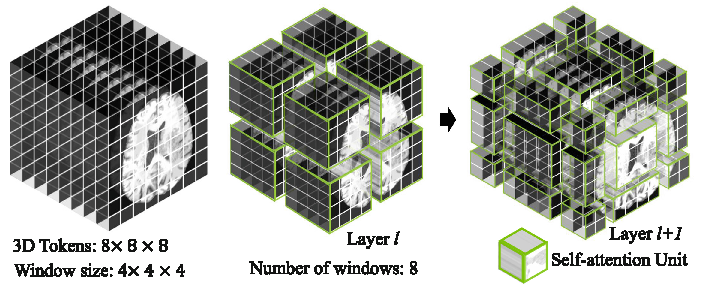
\includegraphics[width=0.48\textwidth]{images/shifted windowing mechanism.pdf}
    \caption{Shifted windowing mechanism}
    \label{fig:shifted_windowing_mechanism}
\end{figure}

\item Decoder: CNN-based Decoder

The decoder follows a U-Net architecture with skip connections from encoder stages i ∈ {0,1,2,3,4} and bottleneck (i=5). At each level:
 
Feature Reshaping: 
            Encoder outputs are reshaped to spatial dimensions: 
            \begin{equation}
                z_i \in R^{\frac{H}{2^i} \times \frac{W}{2^i} \times \frac{D}{2^i} \times C}
            \end{equation}
            
      Residual Processing: 
            Two 3×3×3 conv layers with instance norm (IN) process features\cite{Ulyanov2016InstanceNT}:
            \begin{equation}
                z'_i = \text{Conv3D}(\text{ReLU}(\text{IN}(\text{Conv3D}(z_i))))
            \end{equation}
            
        Upsampling and Fusion: 
            Deconvolution (stride=2) doubles resolution before concatenation:
            \begin{align}
                z_{up} &= \text{Deconv3D}(z'_i) \in R^{\frac{H}{2^{i-1}} \times \frac{W}{2^{i-1}} \times \frac{D}{2^{i-1}} \times C} \\
                z_{fused} &= \text{Concat}(z_{up}, z_{i-1})
            \end{align}
        
  Final Processing:
            Another residual block refines fused features before output:
            
            \begin{equation}
                \hat{z}_i = \text{ResBlock}(z_{fused})
            \end{equation}

       Segmentation Head:
            1×1×1 conv with sigmoid produces voxel-wise probabilities:
            \begin{equation}
                P = \sigma(\text{Conv3D}(\hat{z}_0))
            \end{equation}

The symmetric decoder progressively recovers resolution while integrating multi-scale features through skip connections.
\end{enumerate}

Swin UNETR's 3D spatial advantages were limited by GPU memory constraints, requiring tomogram partitioning that disrupted spatial continuity. Transforming motor coordinates into heatmaps added noise, misaligning with the project's detection focus.


\section{Implementation}
\label{sec:impl}

\subsection{Data description}
The dataset\cite{byu-locating-bacterial-flagellar-motors-2025} used for this project consists of 3D tomograms of biological samples, where the objective is to detect the flagellar motor centers—a critical subcellular structure. Each tomogram is represented as a stack of 2D JPEG slices, forming a volumetric image. The dataset includes flagellar motor coordinates, where, if a motor is present, its 3D position is defined by the motor axis $z$ as the slice index in the tomogram stack, motor axis $y$ as the vertical position (height) within the slice, and motor axis $x$ as the horizontal position (width) within the slice. 
If no motor exists, the submission should indicate this (e.g., with '-1'). Additionally, the dataset provides tomogram metadata, including the array shape, which specifies the dimensions of each tomogram ($z$-axis as the number of slices, $y$-axis as the height of each slice, and $x$-axis as the width of each slice), and voxel spacing, which indicates the physical distance between voxels provided per axis. 
This dataset supports 3D biomedical image analysis, specifically for locating subcellular structures in volumetric data, and the task involves processing 2D slice sequences to infer 3D coordinates, combining computer vision and spatial reasoning.

\subsection{Data preprocessing}
\subsubsection{Data visualization}
To effectively process the tomogram data, we first conducted comprehensive visualization and examination.
Figure \ref{fig:sample_slices} displays representative slices from the training dataset, highlighting the diversity in image quality and structural clarity that our models needed to accommodate.

\begin{figure}[htb]
    \centering
    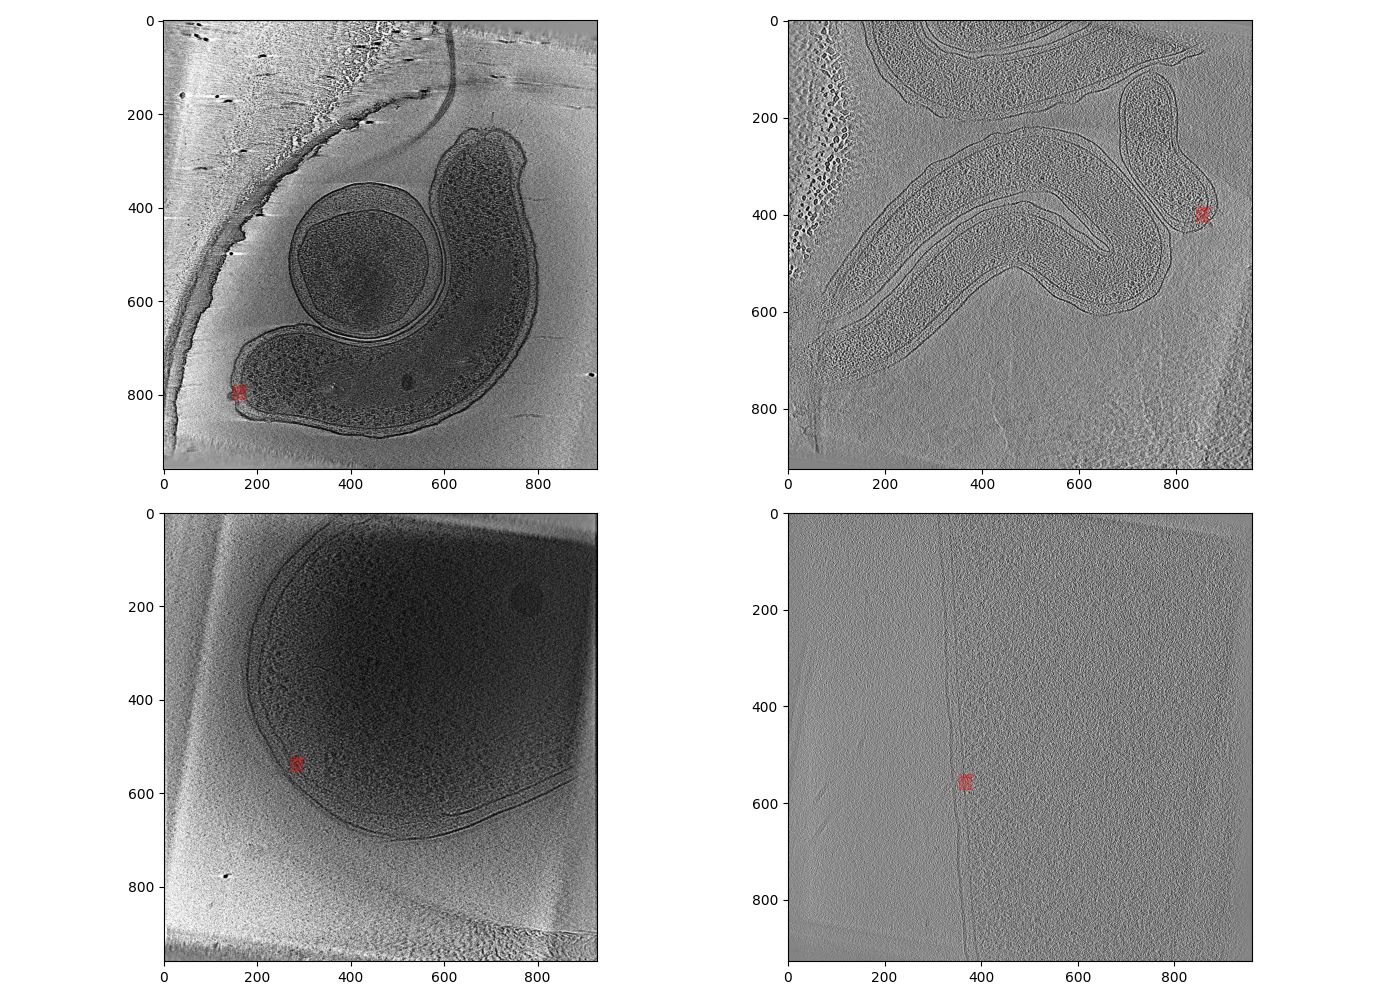
\includegraphics[width=0.5\textwidth]{images/random_training_samples.png}
    \caption{Sample tomographic slices}
    \label{fig:sample_slices}
\end{figure}

My analysis involved examining the statistical distributions of key features across the dataset. Figure \ref{fig:feature_distributions} illustrates the distributions of motor coordinates and tomogram dimensions, revealing important characteristics that informed our modeling approach.

\begin{figure}[htb]
    \centering
    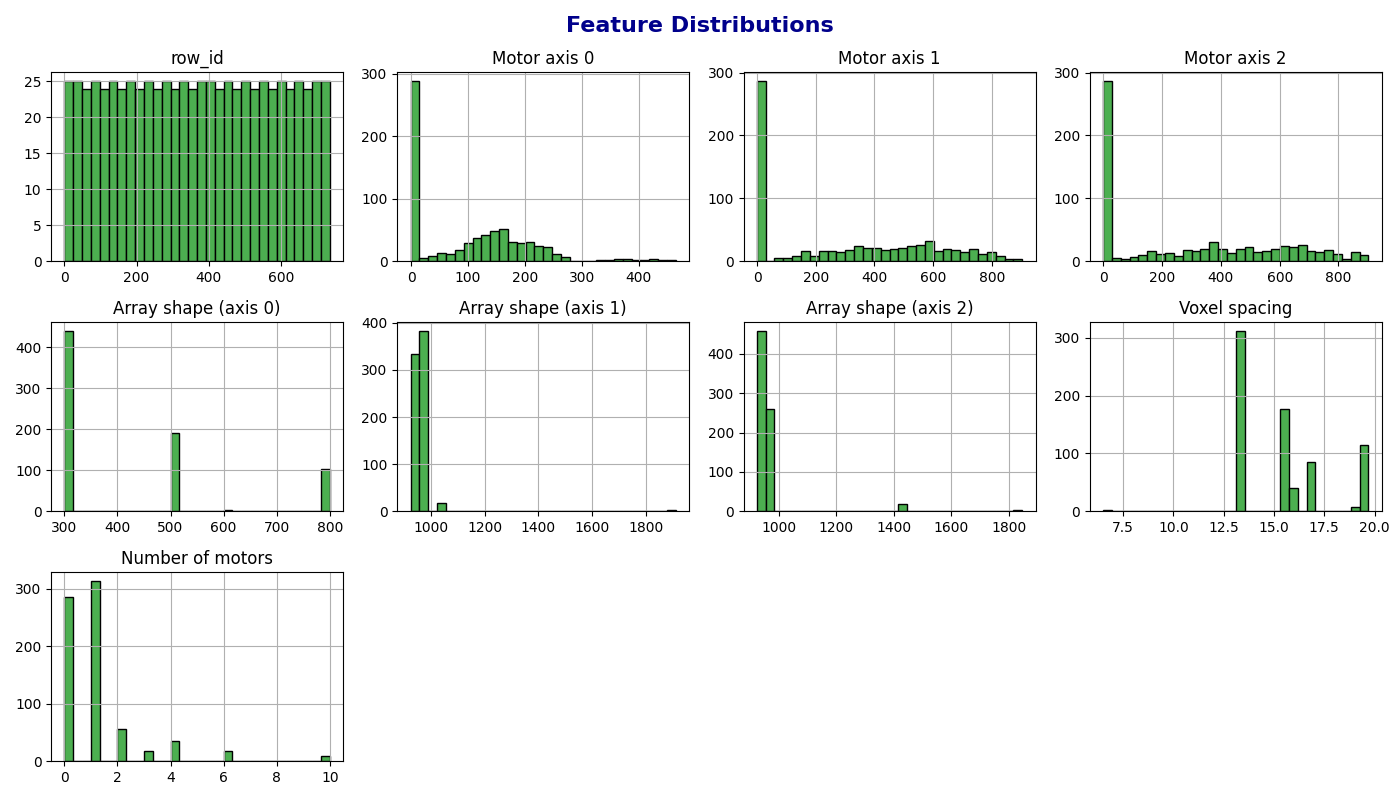
\includegraphics[width=0.48\textwidth]{images/feature_distributions.png}
    \caption{Distributions of key dataset features}
    \label{fig:feature_distributions}
\end{figure}


Further quantitative analysis revealed several important dataset characteristics:

\begin{enumerate}
    \item \textbf{Label quality}: Table \ref{tab:sample_labels} highlights the detailed training labels, which include tomogram IDs, precise 3D motor coordinates, and voxel spacing, ensuring comprehensive annotation for model training.
    \item \textbf{Dimensional variation}: Tomogram dimensions varied considerably across the dataset—Z-axis (slice count): 300-800, X-axis (width): 924-1912, and Y-axis (height): 924-1847—necessitating adaptive processing strategies.
    \item \textbf{Resolution diversity}: Distribution of voxel spacing in Figure \ref{fig:feature_distributions} summarizes the distribution of voxel spacing values, with 13.1, 15.6, and 19.7 being most prevalent, indicating varying levels of detail across samples.
\end{enumerate}

\begin{table}[htb]
    \centering
    \caption{Representative examples from training labels demonstrating data structure}
    \resizebox{\columnwidth}{!}{%
    \begin{tabular}{cccccc}
        \toprule
        Row ID & Tomogram ID & Motor Axis 0 & Motor Axis 1 & Motor Axis 2 & Voxel Spacing \\
        \midrule
        0 & tomo\_003acc & -1.0 & -1.0 & -1.0 & 6.5 \\
        1 & tomo\_00e047 & 169.0 & 546.0 & 603.0 & 15.6 \\
        2 & tomo\_00e463 & 235.0 & 403.0 & 137.0 & 19.7 \\
        3 & tomo\_00e463 & 243.0 & 363.0 & 153.0 & 19.7 \\
        4 & tomo\_00e463 & 222.0 & 379.0 & 144.0 & 19.7 \\
        \bottomrule
    \end{tabular}
    }
    \label{tab:sample_labels}
\end{table}

This analysis informed our subsequent preprocessing decisions, particularly regarding normalization strategies and model input dimensionality requirements.

\subsubsection{Data exploration}
After the initial visualization, we conducted a comprehensive statistical analysis of the dataset to better understand its characteristics and inform our modeling approach.

\begin{table}[htb]
    \centering
    \caption{Statistical summary of key dataset features}
    \resizebox{\columnwidth}{!}{%
    \begin{tabular}{lrrrrrr}
        \toprule
        Statistic & Motor Axis 0 & Motor Axis 1 & Motor Axis 2 & Array Shape Z & Array Shape X & Array Shape Y \\
        \midrule
        count & 737.00 & 737.00 & 737.00 & 737.00 & 737.00 & 737.00 \\
        mean  & 101.86 & 294.85 & 300.82 & 422.65 & 950.21 & 954.82 \\
        std   & 102.21 & 282.33 & 293.37 & 174.34 & 64.86 & 97.23 \\
        min   & -1.00 & -1.00 & -1.00 & 300.00 & 924.00 & 924.00 \\
        25\%  & -1.00 & -1.00 & -1.00 & 300.00 & 928.00 & 928.00 \\
        50\%  & 106.00 & 278.00 & 280.00 & 300.00 & 959.00 & 928.00 \\
        75\%  & 170.00 & 549.00 & 567.00 & 500.00 & 960.00 & 956.00 \\
        max   & 466.00 & 904.00 & 902.00 & 800.00 & 1912.00 & 1847.00 \\
        \bottomrule
    \end{tabular}%
    }
    \label{tab:dataset_statistics}
\end{table}

This statistical analysis revealed several important insights:

\begin{enumerate}
    \item \textbf{Motor presence distribution}: Approximately 46\% of data points have value "-1.0" for motor coordinates, indicating tomograms without motors, which creates a class imbalance challenge.    
    \item \textbf{Spatial distribution}: Analysis of motor positions revealed no strong spatial bias, with motors distributed throughout the volume space, though slightly favoring central regions.
\end{enumerate}

To understand feature relationships, we computed correlations between key variables using Pearson's correlation coefficient. The results, shown in Figure \ref{Fig:correlation_matrix}, indicate weak correlations between motor coordinates and tomogram dimensions, suggesting that motor localization is not strongly influenced by tomogram size.

\begin{figure}[htb]
    \centering
    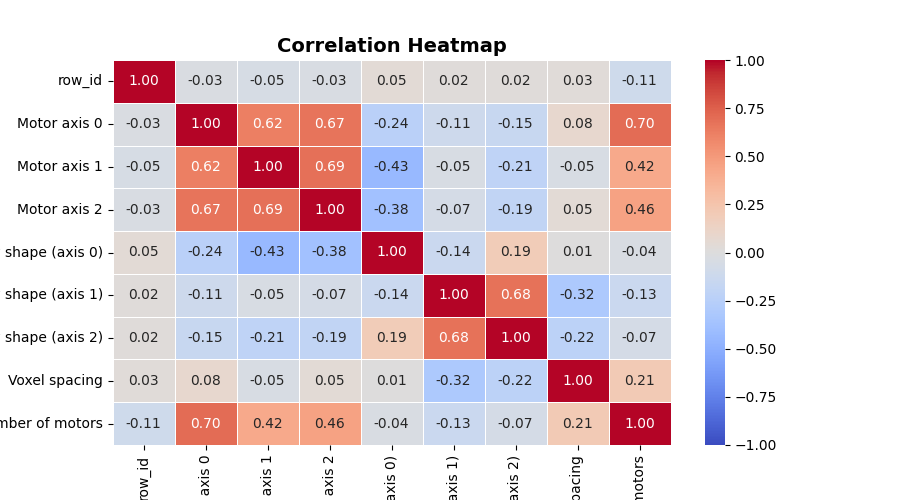
\includegraphics[width=0.48\textwidth]{images/correlation_heatmap.png}
    \caption{Correlation matrix of key dataset features}
    \label{Fig:correlation_matrix}
\end{figure}


These insights directly informed our preprocessing strategies, particularly the need for robust normalization and data augmentation techniques to account for the observed variability.

\subsection{2D model YOLOv8 implementation}

\subsubsection{Dataset preparation}
To train our YOLO-based motor detection model, we developed a robust data preprocessing pipeline. This included extracting 2D slices around annotated motor locations from tomograms, applying percentile-based contrast enhancement for improved clarity, and generating fixed-size bounding boxes centered on motor positions in YOLO-compatible format. We ensured a tomogram-based train/validation split (80\%/20\%) to prevent data leakage, organizing the dataset into the required directory structure with a configuration file for seamless integration into the YOLO framework.

\subsubsection{Model training}
To train the YOLOv8 model for detecting bacterial flagellar motors, we utilized transfer learning by fine-tuning the pretrained YOLOv8n (nano) model, which is optimized for lightweight applications and faster inference. The training process was configured with the following key parameters:

\begin{enumerate}
    \item \textbf{Pretrained Weights:} We initialized the model with pretrained weights, leveraging its robust feature extraction capabilities for object detection tasks.
    \item \textbf{Epochs:} The model was trained for 100 epochs to ensure convergence while avoiding overfitting.
    \item \textbf{Batch Size:} A batch size of 16 was chosen to balance memory usage and training stability.
    \item \textbf{Image Size:} Input images were resized to 640x640 pixels, maintaining a balance between computational efficiency and detection accuracy.
\end{enumerate}

The training process involved optimizing the model using the Adam optimizer with a learning rate scheduler to adaptively adjust the learning rate. Advanced data augmentation techniques, such as mosaic and mixup, were applied to enhance the model's generalization capabilities.

The results of the training process were visualized, as shown in Figure \ref{fig:yolo_training_results}, showing key metrics such as precision, recall, and mAP (mean Average Precision) over the epochs. The training loss and validation loss curves indicated steady convergence, with validation loss stabilizing after approximately 80 epochs. The precision-recall curve demonstrated the model's ability to achieve high recall without significant loss of precision, highlighting its effectiveness in detecting motors across diverse tomographic slices.

\begin{figure}[htb]
    \centering
    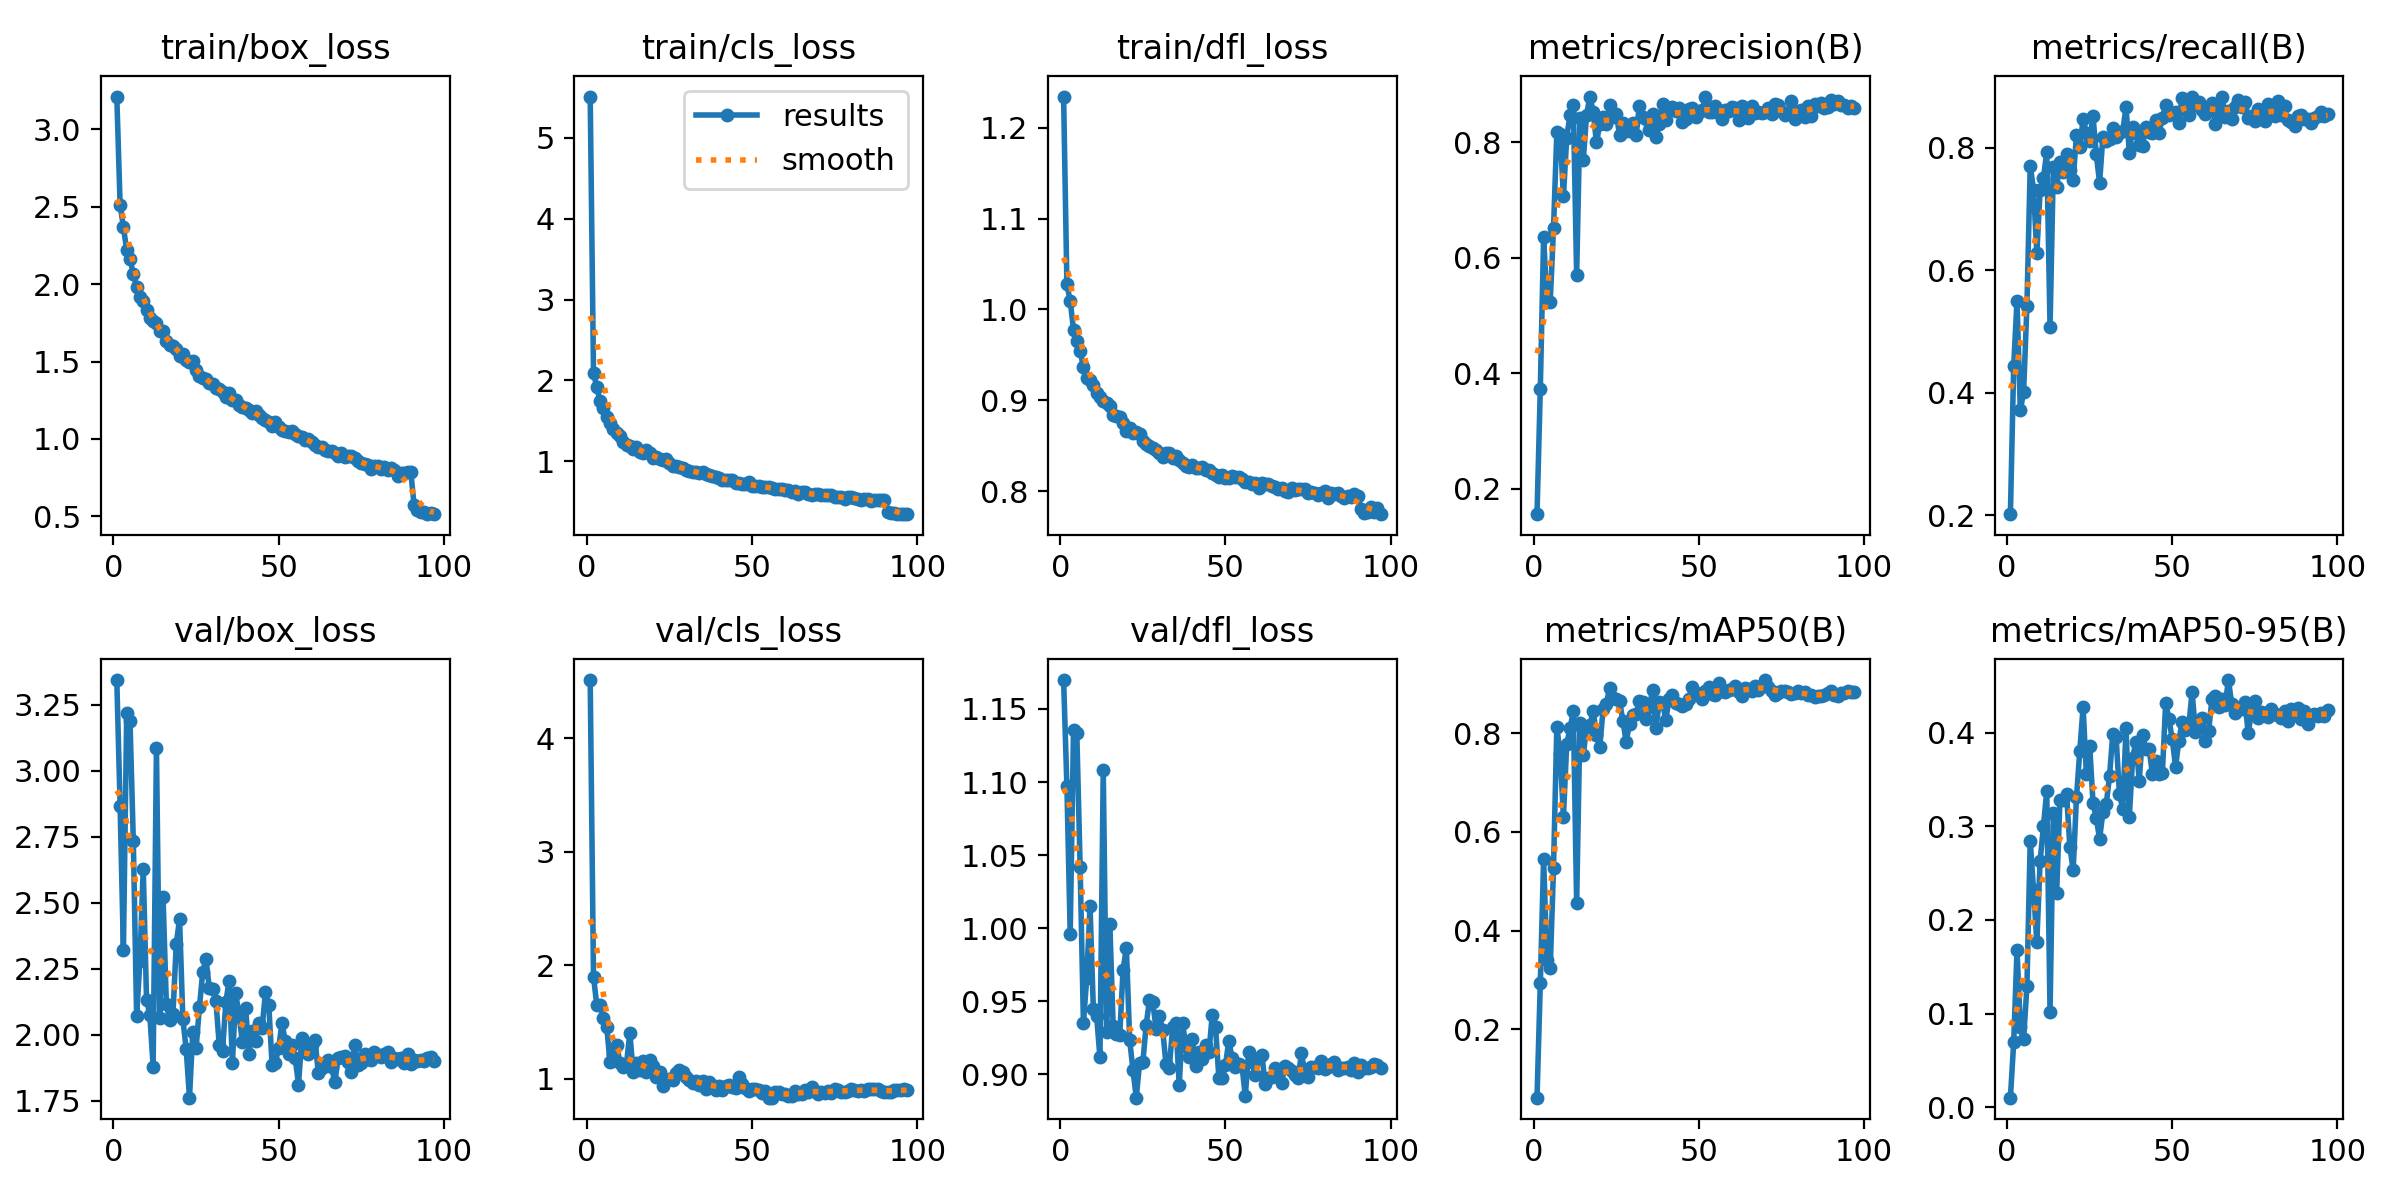
\includegraphics[width=0.48\textwidth]{images/results.png}
    \caption{Training and validation results for YOLOv8 model}
    \label{fig:yolo_training_results}
\end{figure}

\subsection{3D model Swin UNETR implementation}

\subsubsection{Dataset preparation}
To prepare the dataset for the 3D Swin UNETR model, we converted raw tomograms (2D JPEG stacks) into NIfTI (.nii.gz) format. Slices were stacked along the Z-axis to form 3D arrays, normalized using the 2nd and 98th percentiles for consistent intensity scaling. Motor coordinates were normalized relative to tomogram dimensions and converted into 3D heatmaps with Gaussian peaks at motor positions. Tomograms and heatmaps were cropped and resized to \(96 \times 96 \times 96\) voxels for uniform input. Data augmentation, including random flips, rotations, and intensity scaling, was applied to enhance generalization. The processed data can be visualized in 3D using NiiVUE, as shown in Figure \ref{fig:3d_visualization}.

\begin{figure}[htb]
    \centering
    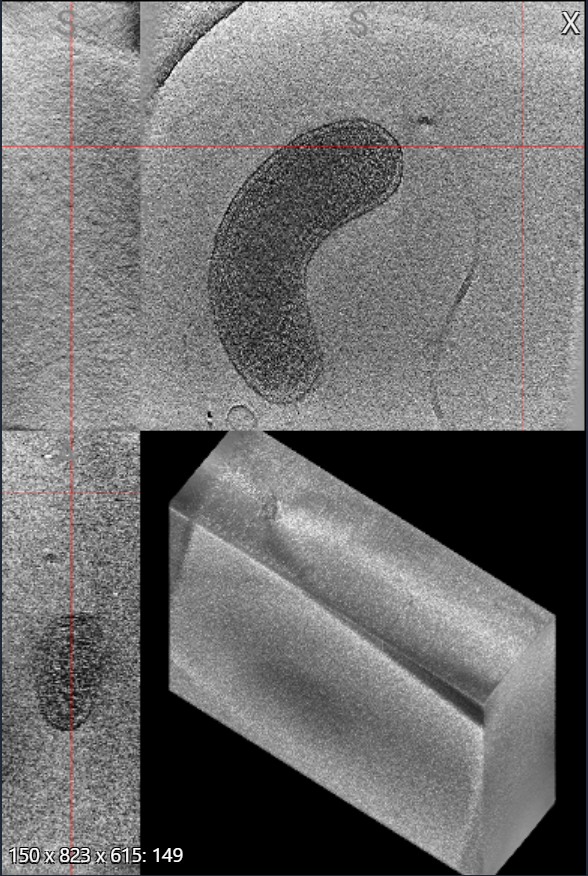
\includegraphics[width=0.3\textwidth]{images/3D view of tomogram.png}
    \caption{3D visualization of tomogram}
    \label{fig:3d_visualization}
\end{figure}

\subsubsection{Model training}
To train the Swin UNETR model for detecting bacterial flagellar motors in 3D tomograms, we implemented a comprehensive training pipeline leveraging the MONAI framework\cite{Cardoso2022MONAIAO}. The training process was configured with the following key parameters:

\begin{enumerate}
    \item \textbf{Loss Function:} Mean Squared Error (MSE) loss was used to measure the difference between predicted heatmaps and ground truth labels, ensuring precise localization of motor centers.
    \item \textbf{Optimizer:} The AdamW optimizer was employed with a learning rate of $1 \times 10^{-4}$ and weight decay of $1 \times 10^{-5}$ to balance convergence speed and generalization.
    \item \textbf{Batch Size:} A batch size of 8 was chosen to maximize GPU utilization while maintaining stable training dynamics.
    \item \textbf{Training Duration:} The model was trained for 50 epochs, with validation performed after each epoch to monitor performance.
\end{enumerate}

The training and validation loss curves, shown in Figures \ref{fig:training_loss} and \ref{fig:validation_loss}, demonstrate steady convergence. The training loss decreased rapidly during the initial epochs, stabilizing after approximately 10 epochs, while the validation loss followed a similar trend, indicating effective generalization.

\begin{figure}[htb]
    \centering
    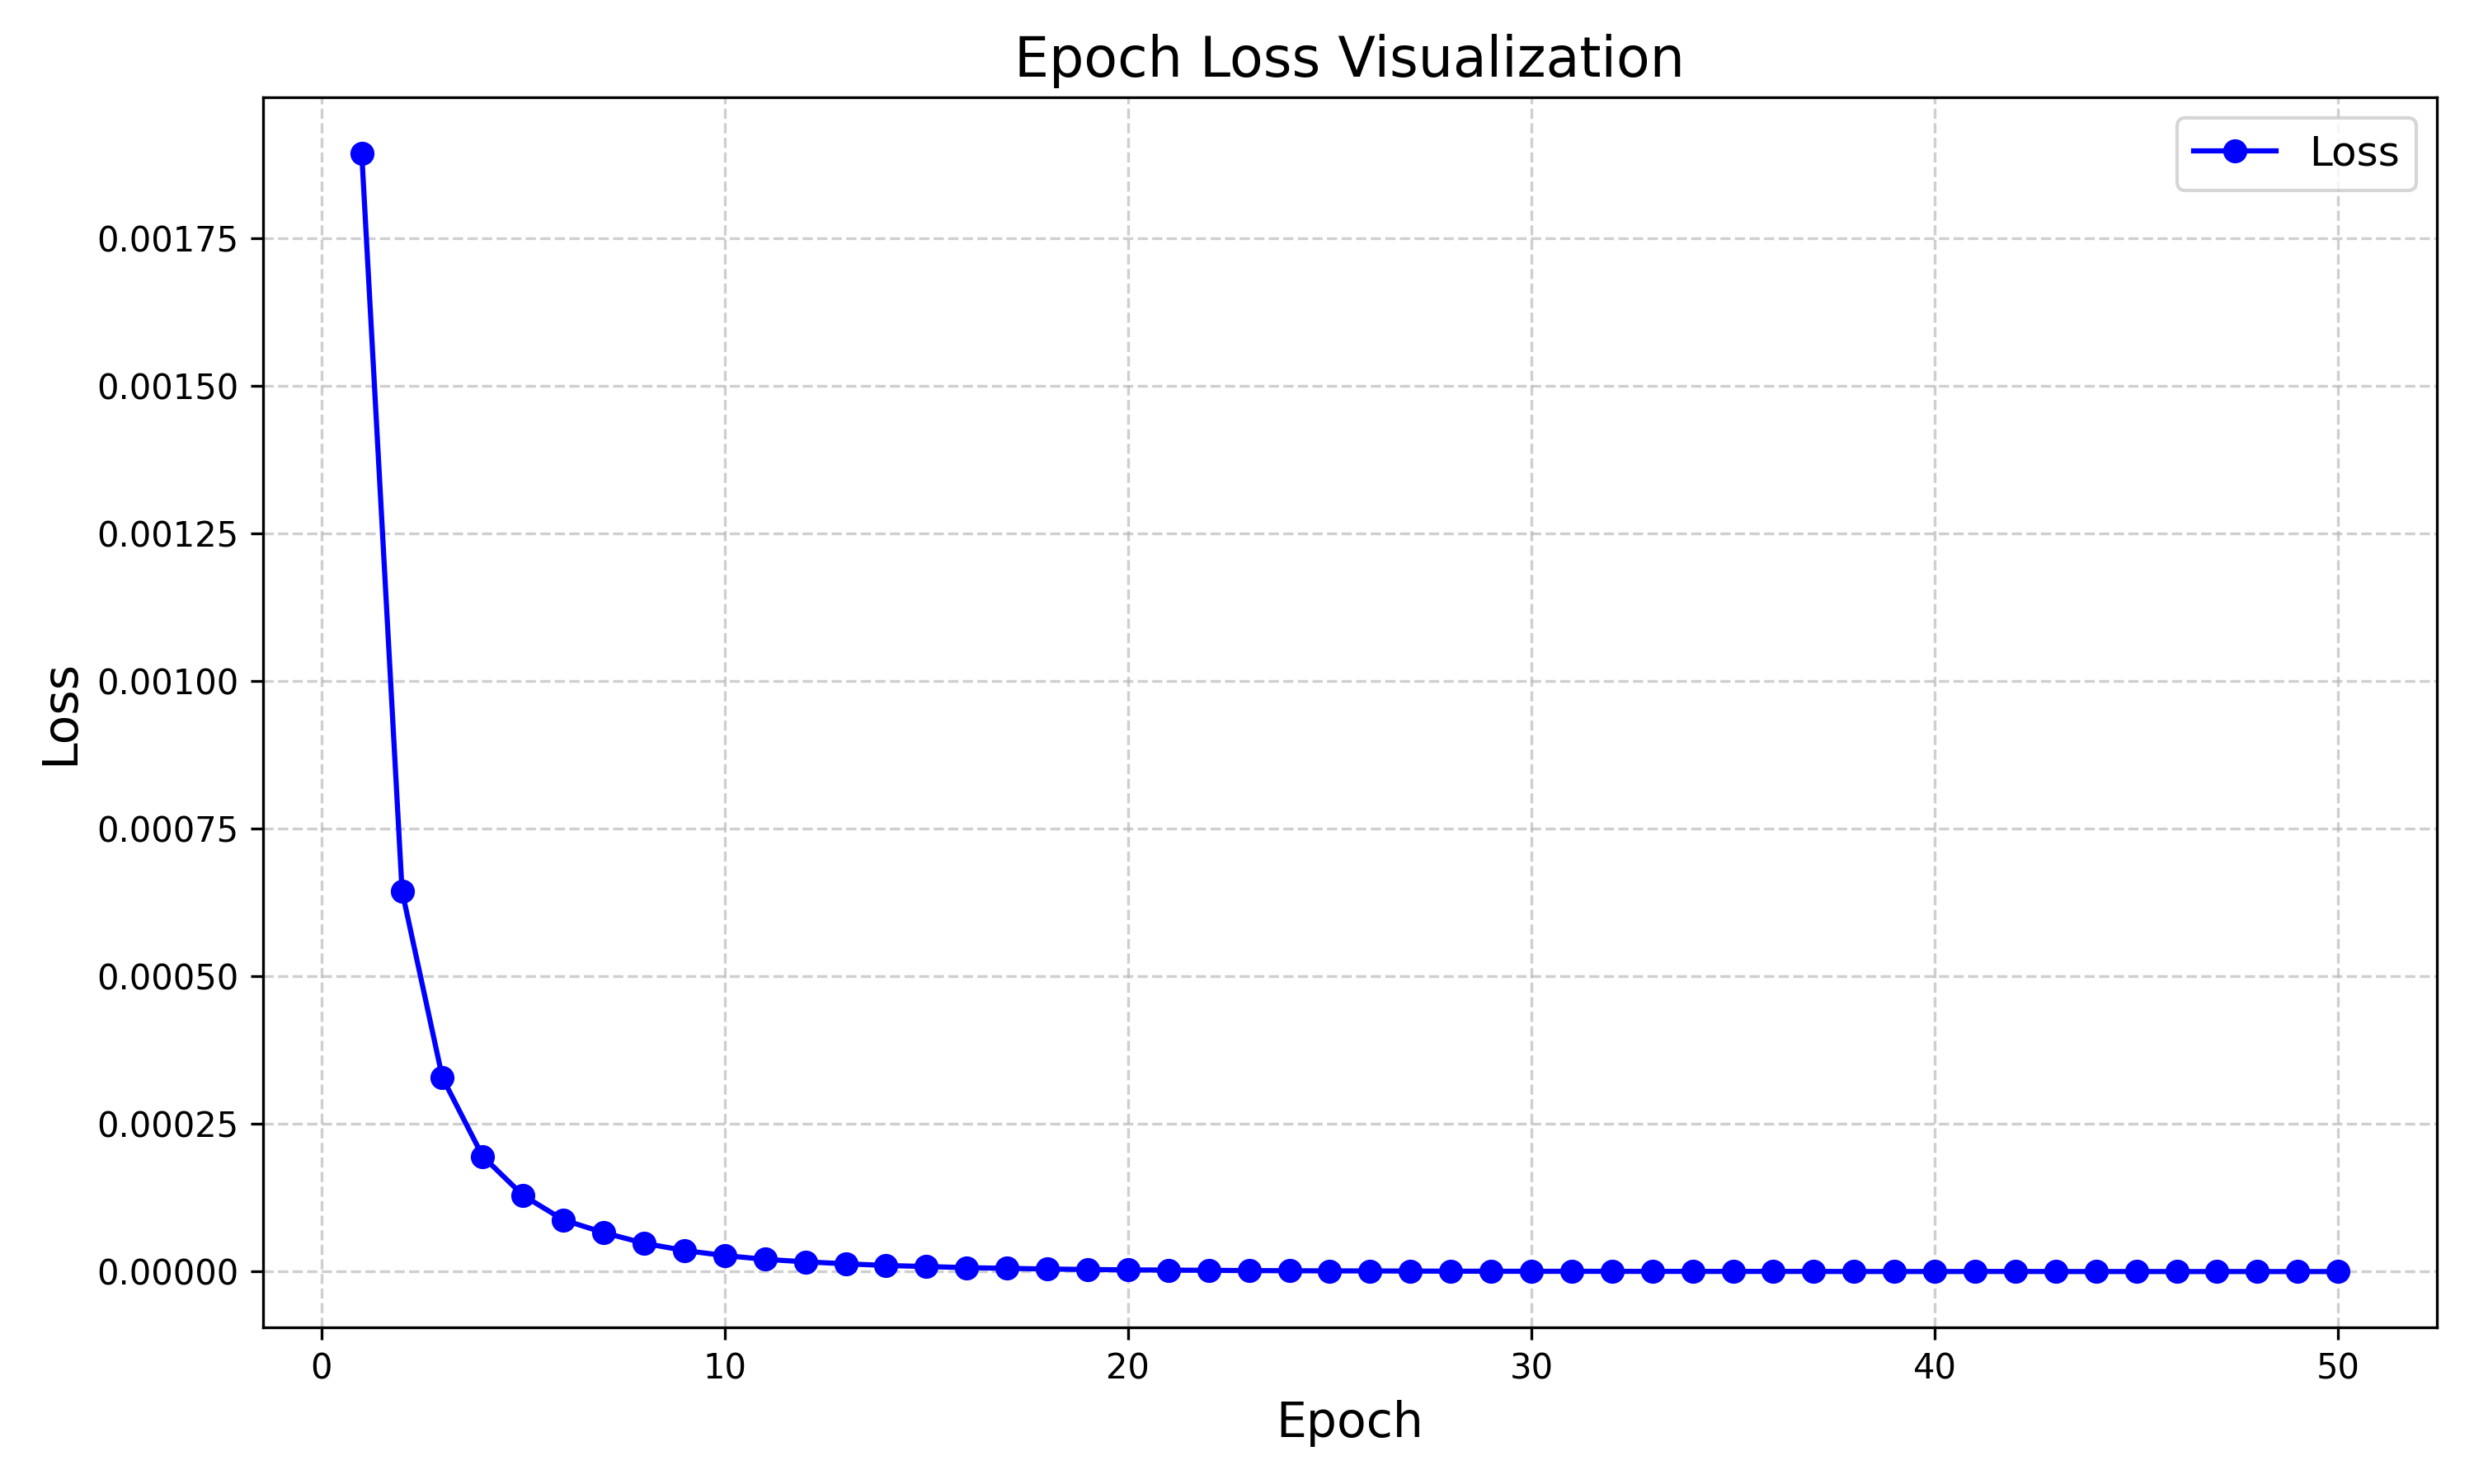
\includegraphics[width=0.48\textwidth]{images/unet_train_epoch_loss_visualization.png}
    \caption{Training loss curve for Swin UNETR model}
    \label{fig:training_loss}
\end{figure}

\begin{figure}[htb]
    \centering
    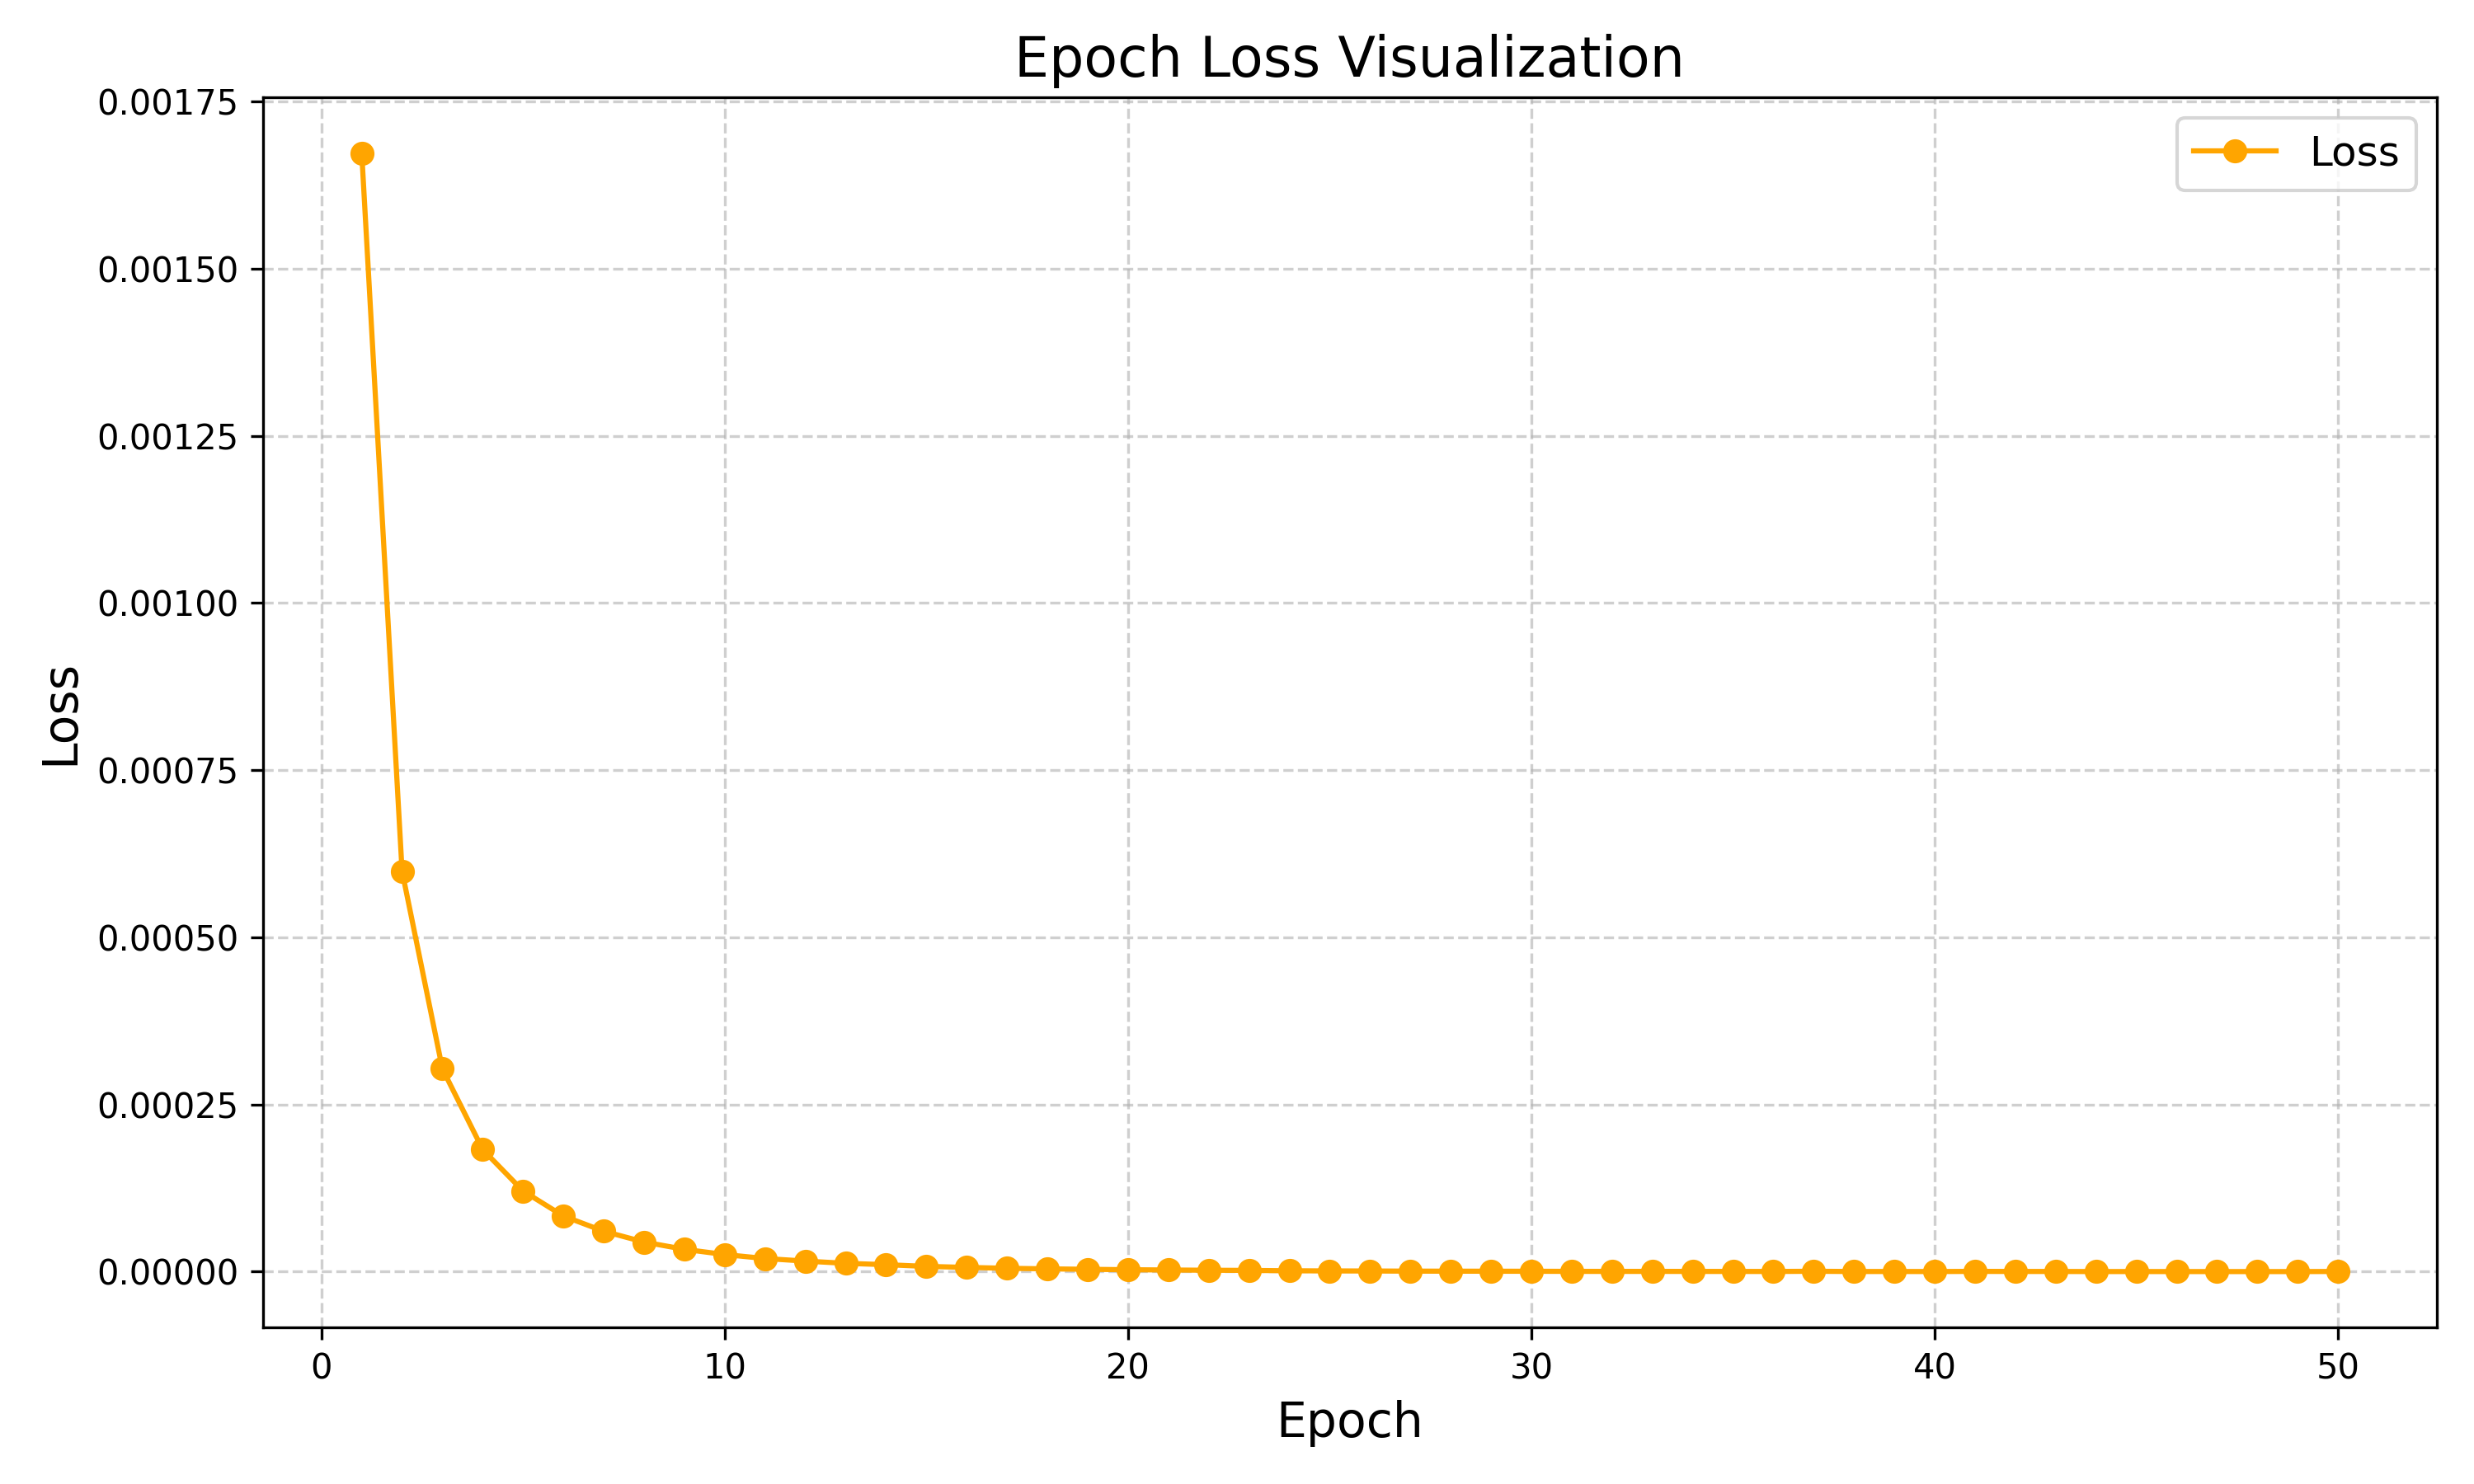
\includegraphics[width=0.48\textwidth]{images/unet_val_epoch_loss_visualization.png}
    \caption{Validation loss curve for Swin UNETR model}
    \label{fig:validation_loss}
\end{figure}

\section{Experimental Results and Analysis}  
\label{sec:results}  

\subsection{Evaluation Metric}

The performance of the models was evaluated using both quantitative metrics and qualitative assessments. The evaluation considered two key aspects: classification accuracy, which determines whether a motor is present, and localization accuracy, which assesses the precision of the predicted motor coordinates.  

Let \(\mathbf{y}\) and \(\hat{\mathbf{y}}\) denote the ground truth and predicted motor axis coordinates, respectively. A prediction is considered correct if the Euclidean distance between \(\mathbf{y}\) and \(\hat{\mathbf{y}}\) is within a predefined threshold \(T = 1000\) Å. Accordingly, we define:  

True Positive (TP): A prediction satisfying  \[\|\mathbf{y} - \hat{\mathbf{y}}\|_2 \leq T.\]
False Negative (FN): A prediction that exceeds the threshold:  
  \[
  \|\mathbf{y} - \hat{\mathbf{y}}\|_2 > T.
  \]  

To evaluate model performance, we use the \(F_{\beta}\)-score, which balances precision and recall. Setting \(\beta=2\) emphasizes recall twice as much as precision:  
\begin{equation}
    F_\beta = (1+\beta^2) \cdot \frac{\text{Precision} \cdot \text{Recall}}{\beta^2 \cdot \text{Precision} + \text{Recall}}.
\end{equation}  
Here, precision and recall are given by  
\[
\text{Precision} = \frac{TP}{TP + FP}, \quad  
\text{Recall} = \frac{TP}{TP + FN}.
\]  

\subsection{Model performance comparison}

\begin{table}[htb]
    \centering
    \caption{Performance metrics for YOLOv8 and Swin UNETR models on the test set}
    \begin{tabular}{lccc}
        \toprule
        Model & Precision & Recall & $F_2$-Score \\
        \midrule
        YOLOv8 & 0.86 & 0.85 & 0.8 \\
        Swin UNETR & 0.65 & 0.63 & 0.6 \\
        \bottomrule
    \end{tabular}
    \label{tab:combined_results}
\end{table}

Table \ref{tab:combined_results} shows that YOLOv8 significantly outperformed Swin UNETR across all metrics. Several factors contributed to this performance gap:
The original task involves detecting specific coordinate points rather than segmenting regions, which inherently favors detection frameworks like YOLOv8. For Swin UNETR implementation, motor coordinate labels had to be transformed into heatmap representations, introducing information distortion. This conversion process—where discrete coordinate points were expanded into Gaussian-centered distributions—created an artificial segmentation problem that deviated from Swin UNETR's optimal use case. The model had to learn to identify these artificially generated heatmap peaks rather than directly predicting coordinate locations.

\begin{figure}[htb]
    \centering
    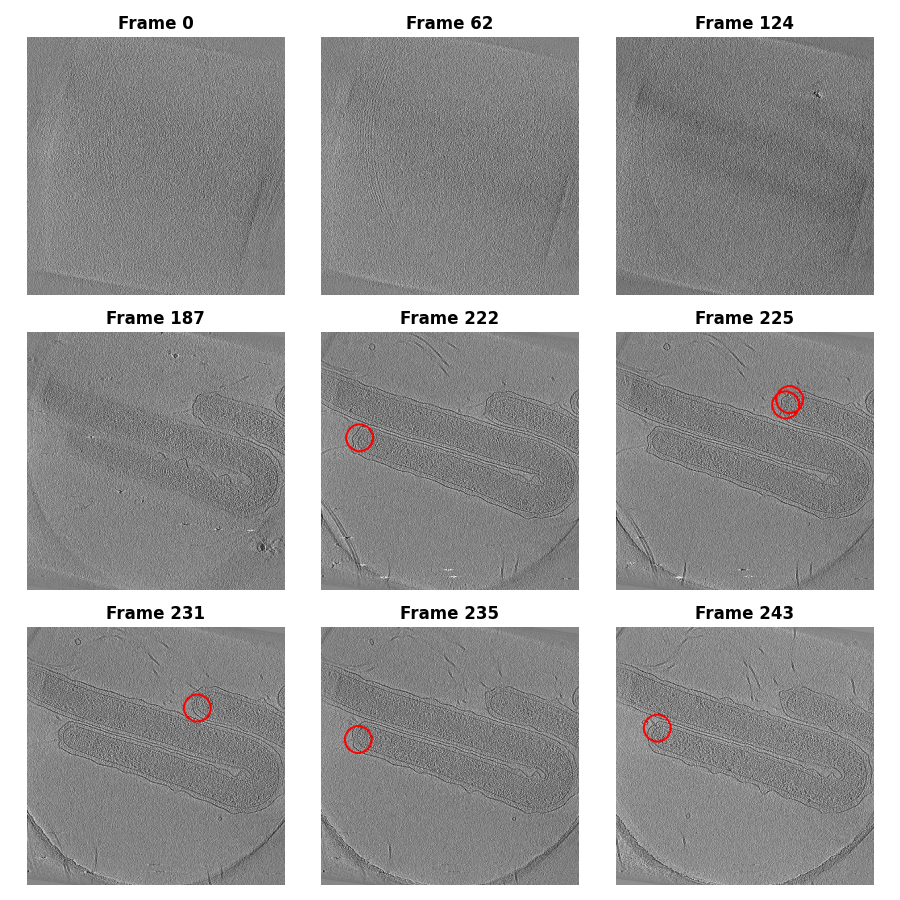
\includegraphics[width=0.48\textwidth]{images/test_sample.png}
    \caption{Test sample with YOLOv8 predictions}
    \label{fig:test_sample}
\end{figure}

On the other hands, The computational requirements of the two models differed substantially:

\begin{enumerate}
    \item \textbf{Parameter count}: Swin UNETR is significantly larger than YOLOv8n, requiring more data and computational resources for optimal training.
    \item \textbf{Training approach}: YOLOv8 benefited from transfer learning, leveraging pre-trained weights that already encoded general visual features. In contrast, Swin UNETR was trained from scratch, requiring more epochs to develop effective feature representations.
    \item \textbf{Training duration}: Due to GPU resource limitations, Swin UNETR was trained for only 50 epochs, likely insufficient for full convergence given its size and lack of pre-training.
\end{enumerate}

Limited GPU memory significantly impacted the 3D approach, as the original tomographic volumes had to be divided into small ($96 \times 96 \times 96$ voxel) patches to fit in available GPU memory, which fragmented spatial context. This partitioning eliminated important long-range dependencies and structural relationships that Swin UNETR was specifically designed to capture through its transformer architecture. Additionally, the partitioning created artificial boundaries, potentially introducing edge artifacts that further complicated the learning process.

% The nature of the task aligned more closely with YOLOv8's design principles:

% \begin{itemize}
%     \item \textbf{Problem formulation}: Flagellar motor detection fundamentally involves locating discrete points in 3D space, which maps cleanly to YOLO's object detection paradigm.
%     \item \textbf{Efficiency in 2D processing}: YOLOv8 efficiently processes individual 2D slices, requiring less memory while maintaining spatial context within each slice.
%     \item \textbf{Sparse annotation handling}: YOLO naturally handles sparse annotations (limited positive samples) through its objectness prediction mechanism, while Swin UNETR must learn to produce mostly-zero heatmaps with isolated peaks.
% \end{itemize}

These results highlight that model selection should consider not only theoretical capabilities but also practical constraints of the specific task, available computational resources, and data representation format. While 3D models theoretically capture more complete spatial relationships in volumetric data, their benefits can be undermined by practical limitations in real-world implementation scenarios.



\section{Conclusion}
\label{sec:conc}

In conclusion, this study presents a comprehensive comparison of two deep learning approaches for detecting bacterial flagellar motors in cryo-ET data: a 2D approach using YOLOv8 and a 3D approach using Swin UNETR. Our experimental results demonstrate that the YOLOv8 model significantly outperforms the Swin UNETR model across all evaluation metrics, achieving an F2-score of 0.8 compared to 0.6 for the 3D approach.

The superior performance of YOLOv8 can be attributed to several factors. First, the problem formulation of detecting discrete coordinate points aligns naturally with YOLO's object detection paradigm. Second, YOLOv8 benefits from transfer learning, leveraging pre-trained weights that already encode general visual features. Additionally, the 2D approach efficiently processes individual slices without the memory constraints faced by volumetric models, allowing it to maintain spatial context while requiring fewer computational resources.

Despite its theoretical advantages in capturing complete 3D spatial relationships, Swin UNETR faced significant practical limitations in our implementation. The necessity to partition large tomographic volumes into small patches due to GPU memory constraints fragmented spatial context and eliminated important long-range dependencies. Furthermore, the conversion of discrete coordinate labels into heatmap representations introduced information distortion, creating an artificial segmentation problem that deviated from Swin UNETR's optimal use case.

These findings highlight an important consideration in model selection: the theoretical capabilities of a model must be balanced against practical constraints of the specific task, available computational resources, and data representation format. While 3D models appear promising for volumetric data analysis, their benefits can be undermined by implementation challenges in real-world scenarios.

Future work could explore hybrid approaches that combine the efficiency of 2D processing with the spatial awareness of 3D models, potentially through sequential 2D-then-3D processing or attention mechanisms that selectively focus on regions of interest. Additionally, investigating more memory-efficient 3D architectures or hierarchical processing strategies could help overcome the current limitations of volumetric approaches. As computational resources continue to improve, the gap between theoretical capabilities and practical implementation of 3D models will likely narrow, potentially shifting the balance in favor of fully volumetric approaches for cryo-ET analysis.



\vfill\pagebreak




% References should be produced using the bibtex program from suitable
% BiBTeX files (here: strings, refs, manuals). The IEEEbib.bst bibliography
% style file from IEEE produces unsorted bibliography list.
% -------------------------------------------------------------------------
\bibliographystyle{IEEEbib}
\bibliography{refs}


\end{document}
